\documentclass[tikz,border=3pt]{standalone}
\usepackage{amsmath,amssymb}
\usepackage[scaled=0.92]{helvet}
\renewcommand{\familydefault}{\sfdefault}
\usepackage{tikz}
\usetikzlibrary{arrows.meta,calc,shadows.blur}
\definecolor{blue}{HTML}{2A78D6}
\definecolor{bluebg}{HTML}{EEF4FC}
\definecolor{green}{HTML}{3A9E4F}
\definecolor{greenbg}{HTML}{EDF7EF}
\definecolor{navy}{HTML}{104281}
\definecolor{navybg}{HTML}{E9EEF6}
\definecolor{ink}{HTML}{22303C}
\definecolor{muted}{HTML}{66727E}
\definecolor{edge}{HTML}{D6DEE6}

\tikzset{
  cardbox/.style={rounded corners=3pt, fill=white, draw=edge, line width=0.5pt,
                  blur shadow={shadow blur steps=6, shadow xshift=0pt, shadow yshift=-0.6mm, shadow opacity=12}},
  flow/.style={-{Latex[length=2.2mm,width=1.8mm]}, line width=0.9pt, color=muted!80},
  feed/.style={-{Latex[length=2.2mm,width=1.8mm]}, line width=0.9pt, color=green}}

% \card{name}{x}{y}{accent}{soft}{number}{title}{icon code}{body}
\newcommand{\card}[9]{%
  \node[cardbox, anchor=north west, minimum width=42mm, minimum height=40mm] (#1) at (#2mm,#3mm) {};
  \fill[#4, rounded corners=1.5pt] ($(#1.north west)+(3mm,0.6mm)$) rectangle ($(#1.north east)+(-3mm,-0.6mm)$);
  \node[circle, draw=#4, fill=#5, line width=0.6pt, minimum size=5mm, inner sep=0pt,
        font=\bfseries\footnotesize, text=#4] (#1n) at ($(#1.north west)+(5.5mm,-5.5mm)$) {#6};
  \node[anchor=west, font=\bfseries\small, text=ink] at ($(#1n.east)+(1.2mm,0)$) {#7};
  \draw[edge, line width=0.5pt] ($(#1.north west)+(2.5mm,-10mm)$) -- ($(#1.north east)+(-2.5mm,-10mm)$);
  \begin{scope}[shift={($(#1.north)+(0,-14.5mm)$)}, #4, line width=0.8pt]#8\end{scope}
  \node[anchor=north, text width=39mm, align=center, font=\footnotesize, text=ink] at ($(#1.north)+(0,-19mm)$) {#9};
}
\newcommand{\pill}[2]{\tikz[baseline=(p.base)]\node[fill=#1, rounded corners=4pt, inner xsep=4pt, inner ysep=1.5pt](p){#2};}

\begin{document}
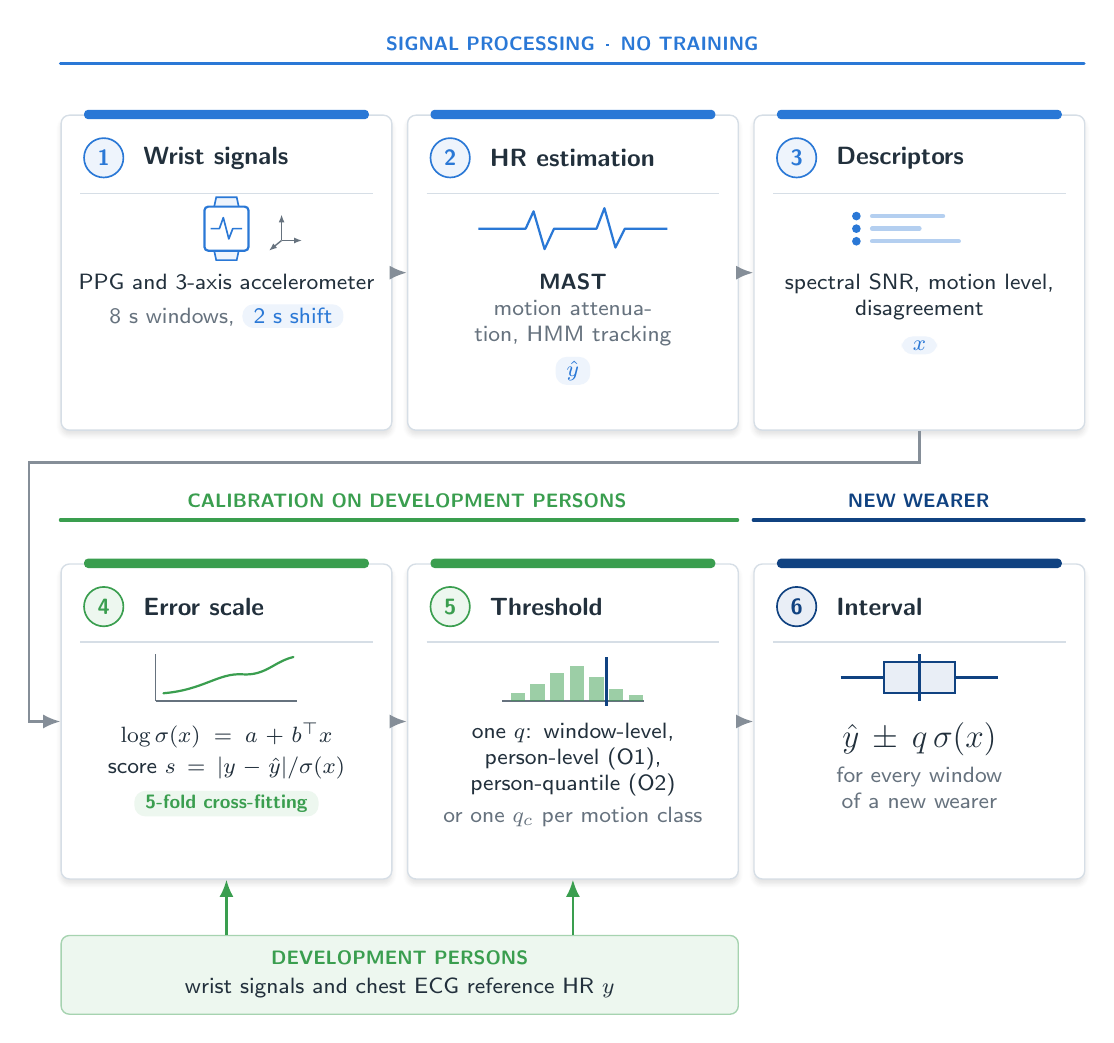
\begin{tikzpicture}
% phase banners
\node[font=\bfseries\scriptsize, text=blue] at (65mm,9mm) {SIGNAL PROCESSING \,\textperiodcentered\, NO TRAINING};
\draw[blue, line width=1.2pt, line cap=round] (0,6.5mm) -- (130mm,6.5mm);
\node[font=\bfseries\scriptsize, text=green] at (44mm,-49mm) {CALIBRATION ON DEVELOPMENT PERSONS};
\draw[green, line width=1.2pt, line cap=round] (0,-51.5mm) -- (86mm,-51.5mm);
\node[font=\bfseries\scriptsize, text=navy] at (109mm,-49mm) {NEW WEARER};
\draw[navy, line width=1.2pt, line cap=round] (88mm,-51.5mm) -- (130mm,-51.5mm);

% row 1
\card{in}{0}{0}{blue}{bluebg}{1}{Wrist signals}
  {\draw[fill=bluebg, line width=0.6pt] (-1.6mm,2.6mm) -- (-1.3mm,4mm) -- (1.3mm,4mm) -- (1.6mm,2.6mm);\draw[fill=bluebg, line width=0.6pt] (-1.6mm,-2.6mm) -- (-1.3mm,-4mm) -- (1.3mm,-4mm) -- (1.6mm,-2.6mm);\draw[fill=white, rounded corners=1.4pt, line width=0.8pt] (-2.8mm,-2.8mm) rectangle (2.8mm,2.8mm);\draw[line width=0.6pt, line join=round] (-2mm,0) -- (-0.9mm,0) -- (-0.4mm,1.4mm) -- (0.3mm,-1.3mm) -- (0.8mm,0) -- (2mm,0);\begin{scope}[shift={(7mm,0)}, line width=0.5pt, muted]\draw[-{Latex[length=1mm]}] (0,-1.5mm) -- (0,1.8mm); \draw[-{Latex[length=1mm]}] (0,-1.5mm) -- (2.6mm,-1.5mm); \draw[-{Latex[length=1mm]}] (0,-1.5mm) -- (-1.6mm,-2.8mm); \end{scope}}
  {PPG and 3-axis accelerometer\\[3pt] {\color{muted}8~s windows,} \pill{bluebg}{\color{blue}2~s shift}}
\card{est}{44}{0}{blue}{bluebg}{2}{HR estimation}
  {\draw[line join=round] (-12mm,0) -- (-6mm,0) -- (-5mm,2.2mm) -- (-3.6mm,-2.6mm) -- (-2.4mm,0) -- (3mm,0) -- (4mm,2.6mm) -- (5.4mm,-2.4mm) -- (6.6mm,0) -- (12mm,0);}
  {\textbf{MAST}\\ {\color{muted}motion attenuation, HMM tracking}\\[3pt] \pill{bluebg}{\color{blue}$\hat y$}}
\card{desc}{88}{0}{blue}{bluebg}{3}{Descriptors}
  {\foreach \i/\w in {0/9,1/6,2/11} {\fill (-8mm,1.6mm-1.6mm*\i) circle (0.55mm); \draw[line width=1.6pt, opacity=0.35, line cap=round] (-6mm,1.6mm-1.6mm*\i) -- (-6mm+\w mm,1.6mm-1.6mm*\i);}}
  {spectral SNR, motion level,\\ disagreement\\[3pt] \pill{bluebg}{\color{blue}$x$}}

% row 2
\card{scale}{0}{-57}{green}{greenbg}{4}{Error scale}
  {\draw[line width=0.5pt, muted] (-9mm,-3mm) -- (9mm,-3mm); \draw[line width=0.5pt, muted] (-9mm,-3mm) -- (-9mm,3mm); \draw[line cap=round] (-8mm,-2mm) .. controls (-3mm,-1.6mm) and (-1mm,0.6mm) .. (2mm,0.4mm) .. controls (5mm,0.2mm) and (6mm,2mm) .. (8.5mm,2.6mm);}
  {$\log\sigma(x) = a + b^{\top}x$\\[2pt] score $s = |y-\hat y|/\sigma(x)$\\[3pt] \pill{greenbg}{\color{green}\scriptsize\bfseries 5-fold cross-fitting}}
\card{cal}{44}{-57}{green}{greenbg}{5}{Threshold}
  {\draw[line width=0.5pt, muted] (-9mm,-3mm) -- (9mm,-3mm); \foreach \x/\h in {-7/1,-4.5/2.2,-2/3.6,0.5/4.4,3/3,5.5/1.6,8/0.8} \fill[opacity=0.5] (\x mm-0.9mm,-3mm) rectangle (\x mm+0.9mm,-3mm+\h mm); \draw[navy, line width=1pt] (4.3mm,-3.6mm) -- (4.3mm,2.6mm);}
  {one $q$: window-level,\\ person-level (O1), person-quantile (O2)\\[2pt] {\color{muted}or one $q_c$ per motion class}}
\card{out}{88}{-57}{navy}{navybg}{6}{Interval}
  {\draw (-10mm,0) -- (10mm,0); \draw[fill=navybg, line width=0.7pt] (-4.5mm,-2mm) rectangle (4.5mm,2mm); \draw[line width=1.1pt] (0,-3mm) -- (0,3mm);}
  {\large$\hat y \pm q\,\sigma(x)$\\[3pt] \footnotesize{\color{muted}for every window of a new wearer}}

% flows
\draw[flow] (in.east) -- (est.west);
\draw[flow] (est.east) -- (desc.west);
\draw[flow] (desc.south) -- ++(0,-4mm) -| ($(scale.west)+(-4mm,0)$) -- (scale.west);
\draw[flow] (scale.east) -- (cal.west);
\draw[flow] (cal.east) -- (out.west);

% development persons
\node[anchor=north, rounded corners=3pt, fill=greenbg, draw=green!45, line width=0.5pt,
      minimum width=86mm, minimum height=10mm, align=center, font=\footnotesize, text=ink] (dev)
      at ($(scale.south west)!0.5!(cal.south east)+(0,-7mm)$)
      {{\color{green}\bfseries\scriptsize DEVELOPMENT PERSONS}\\[1pt] wrist signals and chest ECG reference HR $y$};
\draw[feed] (dev.north -| scale.south) -- (scale.south);
\draw[feed] (dev.north -| cal.south) -- (cal.south);
\end{tikzpicture}
\end{document}
